\chapter{Исследовательский раздел}

В данном разделе будут приведены: пример работы программы, постановка эксперимента и сравнительный анализ алгоритмов на основе полученных данных.

\section{Демонстрация работы программы}


На рисунке \ref{img:program} представлена демонстрация работы разработанного программного обеспечения, а именно показаны результаты сортировки массива $[3, 5, -3, 1, 2, 4, -6, 2]$.

\includeimage
{program} % Имя файла без расширения (файл должен быть расположен в директории inc/img/)
{f} % Обтекание (без обтекания)
{h} % Положение рисунка (см. figure из пакета float)
{0.65\textwidth} % Ширина рисунка
{Демонстрация работы программы при сортировке массива} % Подпись рисунка

\clearpage


\section{Технические характеристики}

Технические характеристики компьютера, на котором проводился замерный эксперимент:
\begin{itemize}
	\item процессор Intel Core i5-10400F (6 ядер)~\cite{intel};
	\item 16 Гб оперативная память DDR4;
	\item операционная система Windows 10 Pro~\cite{windows}.
\end{itemize}

Во время проведения исследования компьютер был нагружен только системными приложениями и целевой программой.

\section{Время выполнения реализаций алгоритмов}

Результаты замеров времени выполнения реализаций алгоритмов сортировок приведены в таблицах \ref{tbl:time_measurements} -- \ref{tbl:time_measurements_rand}.
Замеры времени проводились на массивах одного размера и усреднялись для каждого набора одинаковых экспериментов.

В таблицах \ref{tbl:time_measurements} -- \ref{tbl:time_measurements_rand} используются следующие обозначения: 
\begin{itemize}
	\item Блочная --- реализация алгоритма блочной сортировки;
	\item Быстрая --- реализация алгоритма быстрой сортировки;
	\item Выбором --- реализация алгоритма сортировки выбором.
\end{itemize}

\begin{table}[h]
	\begin{center}
		\begin{threeparttable}
			\captionsetup{justification=raggedright,singlelinecheck=off}
			\caption{Время работы реализации алгоритмов на неотсортированных массивах (в мс)}
			\label{tbl:time_measurements}
			\begin{tabular}{|c|c|c|c|}
				\hline
				Размер массива & Блочная & Быстрая & Выбором \\
				\hline
				100 &$ 0.078 $&$ 0.125 $&$ 0.203 $\\
				\hline
				200 &$ 0.203 $&$ 0.266 $&$ 0.906 $\\
				\hline
				300 &$ 0.406 $&$ 0.500 $&$ 1.781 $\\
				\hline
				400 &$ 0.766 $&$ 0.547 $&$ 3.484 $\\
				\hline
				500 &$ 1.078 $&$ 0.734 $&$ 5.625 $\\
				\hline
				600 &$ 1.391 $&$ 0.891 $&$ 7.813 $\\
				\hline
				700 &$ 1.813 $&$ 1.156 $&$ 10.609 $\\
				\hline
				800 &$ 2.234 $&$ 1.250 $&$ 14.250 $\\
				\hline
				900 &$ 2.984 $&$ 1.297 $&$ 18.063 $\\
				\hline
				1000 &$ 3.734 $&$ 1.500 $&$ 22.516 $\\
				\hline
			\end{tabular}
		\end{threeparttable}
	\end{center}
\end{table}

\begin{table}[h]
	\begin{center}
		\begin{threeparttable}
			\captionsetup{justification=raggedright,singlelinecheck=off}
			\caption{Время работы реализации алгоритмов на отсортированных в обратном порядке массивах (в мс)}
			\label{tbl:time_measurements_sorted}
			\begin{tabular}{|c|c|c|c|}
				\hline
				Размер массива & Блочная & Быстрая & Выбором \\
				\hline
				100 &$ 0.078 $&$ 0.125 $&$ 0.203 $\\
				\hline
				200 &$ 0.203 $&$ 0.250 $&$ 0.766 $\\
				\hline
				300 &$ 0.406 $&$ 0.391 $&$ 1.938 $\\
				\hline
				400 &$ 0.641 $&$ 0.547 $&$ 3.348 $\\
				\hline
				500 &$ 0.969 $&$ 0.688 $&$ 5.375 $\\
				\hline
				600 &$ 1.328 $&$ 0.875 $&$ 7.609 $\\
				\hline
				700 &$ 1.750 $&$ 1.047 $&$ 10.641 $\\
				\hline
				800 &$ 2.609 $&$ 1.141 $&$ 14.047 $\\
				\hline
				900 &$ 2.938 $&$ 1.250 $&$ 17.828 $\\
				\hline
				1000 &$ 3.719 $&$ 1.438 $&$ 22.266 $\\
				\hline
			\end{tabular}
		\end{threeparttable}
	\end{center}
\end{table}

\begin{table}[h]
	\begin{center}
		\begin{threeparttable}
			\captionsetup{justification=raggedright,singlelinecheck=off}
			\caption{Время работы реализации алгоритмов на отсортированных массивах (в мс)}
			\label{tbl:time_measurements_rand}
			\begin{tabular}{|c|c|c|c|}
				\hline
				Размер массива & Блочная & Быстрая & Выбором \\
				\hline
				100 &$ 0.063 $&$ 0.109 $&$ 0.203 $\\
				\hline
				200 &$ 0.203 $&$ 0.313 $&$ 0.828 $\\
				\hline
				300 &$ 0.391 $&$ 0.438 $&$ 1.859 $\\
				\hline
				400 &$ 0.641 $&$ 0.578 $&$ 3.453 $\\
				\hline
				500 &$ 1.000 $&$ 0.688 $&$ 5.313 $\\
				\hline
				600 &$ 1.313 $&$ 0.859 $&$ 7.906 $\\
				\hline
				700 &$ 1.891 $&$ 1.031 $&$ 10.469 $\\
				\hline
				800 &$ 2.281 $&$ 1.125 $&$ 13.813 $\\
				\hline
				900 &$ 2.938 $&$ 1.313 $&$ 18.109 $\\
				\hline
				1000 &$ 3.438 $&$ 1.438 $&$ 22.422 $\\
				\hline
			\end{tabular}
		\end{threeparttable}
	\end{center}
\end{table}

\clearpage
На рисунках \ref{pic:random} -- \ref{pic:sorted} изображены графики зависимостей времени выполнения реализаций сортировок от размеров массивов.

\begin{figure}[H]
	\centering
	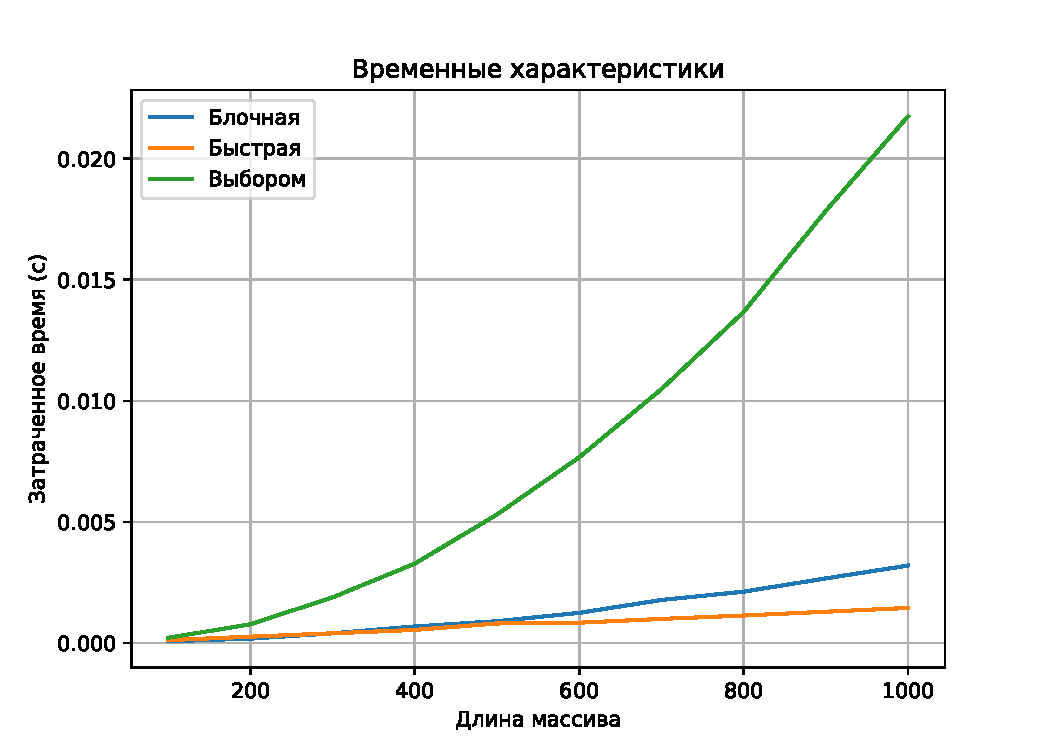
\includegraphics[scale=0.62]{assets/plots/cpu-random.pdf}
	\caption{Сравнение реализаций алгоритмов по времени выполнения на неотсортированных массивах}
	\label{pic:random}
\end{figure}

\newpage

\begin{figure}[H]
	\centering
	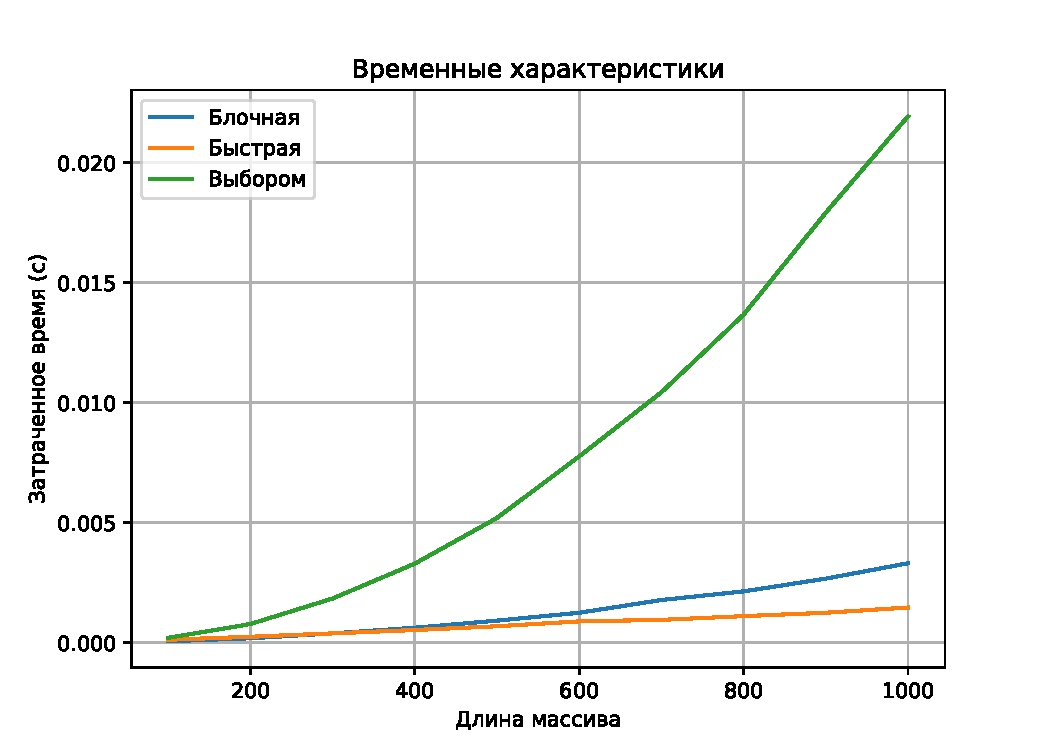
\includegraphics[scale=0.62]{assets/plots/cpu-reversed.pdf}
	\caption{Сравнение реализаций алгоритмов по времени выполнения на отсортированных в обратном порядке массивах}
	\label{pic:reversed}
\end{figure}

\newpage

\begin{figure}[H]
	\centering
	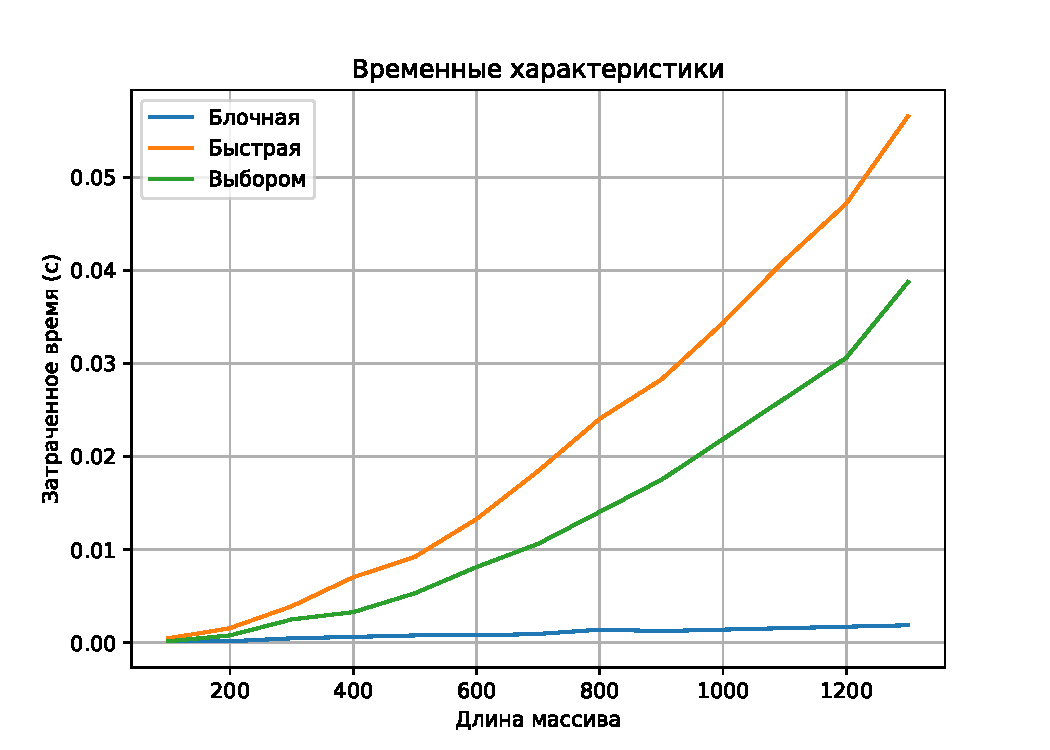
\includegraphics[scale=0.62]{assets/plots/cpu-sorted.pdf}
	\caption{Сравнение реализаций алгоритмов по времени выполнения на отсортированных массивах}
	\label{pic:sorted}
\end{figure}

\clearpage

\section{Затраты по памяти реализаций алгоритмов}

Введем следующие обозначения:
\begin{itemize}
	\item $\text{size}(a)$~--- функция, вычисляющая размер входного параметра a в байтах;
	\item $int$~--- целочисленный тип данных.
\end{itemize}

Теоретически оценим объем используемой алгоритмами памяти при сортировке массива размером $N$.

\subsection{Блочная сортировка}

Оценка используемой блочной сортировкой памяти приведена в формуле

\begin{equation}
	M_{BlockSort} = 5 \cdot \text{size}(int) + N \cdot \text{size}(int) + 8
\end{equation}
где
\begin{itemize}
	\item $5 \cdot \text{size}(int)$~--- дополнительные переменные;
	\item $N \cdot \text{size}(int)$~--- массив блоков;
	\item $8$~--- указатель на массив, переданный в качестве параметра.
\end{itemize}

\subsection{Быстрая сортировка}

Оценка используемой быстрой сортировкой памяти приведена в формуле

\begin{equation}
	\label{eqn:mem-qsort}
	M_{QuickSort} = M_{call} \cdot
	\begin{cases}
		\log_2{N}, & \text{лучший случай}, \\
		N, & \text{худший случай}
	\end{cases}
\end{equation}
где
\begin{itemize}
	\item $M_{call} = (8 + 3 \cdot \text{size}(int) + 8$~--- память, затрачиваемая на один рекурсивный вызов ($8$~--- адрес возврата, $3 \cdot \text{size}(int)$~---дополнительные переменные, $8$~--- указатель на массив);
	\item $\log_2{N}$~--- глубина стека вызовов в лучшем случае;
	\item $N$~--- глубина стека вызовов в худшем случае.
\end{itemize}

Тогда итоговая формула
\begin{equation}
	\label{eqn:mem-qsort}
	M_{QuickSort} = (8 + 3 \cdot \text{size}(int) + N \cdot \text{size}(int)) \cdot
	\begin{cases}
		\log_2{N}, & \text{лучший случай}, \\
		N, & \text{худший случай}
	\end{cases}
\end{equation}

\subsection{Сортировка выбором}

Оценка используемой сортировкой выбором памяти приведена в формуле

\begin{equation}
	M_{ChoiceSort} = 3 \cdot \text{size}(int) + 8
\end{equation}
где
\begin{itemize}
	\item $3 \cdot \text{size}(int)$~--- дополнительные переменные;
	\item $8$~--- указатель на массив, переданный в качестве параметра.
\end{itemize}


\section*{Вывод}

В результате замеров времени выполнения реализаций различных алгоритмов было выявлено, что для массивов длиной 1000, отсортированных в обратном порядке, реализация алгоритма быстрой сортировки по времени оказалась в 2.59 раз лучше, чем реализация блочной сортировки, и в 15.49 раз лучше реализации сортировки выбором. 
В свою очередь, реализация блочной сортировки оказалась лучше в 5.99 раз по времени выполнения, чем реализация  сортировки выбором.

Для отсортированных массивов длиной 1000 реализация быстрой сортировки оказалась лучше по времени в 2.39 раз, чем реализация блочной сортировки, и в 15.6 раз лучше, чем реализация сортировки выбором. 
В свою очередь, реализация блочной сортировки оказалась лучше в 6.52 раза по времени выполнения, чем реализация сортировки выбором.

Для случайно упорядоченных массивов длиной 1000 реализация быстрой сортировки оказалась лучше по времени в 2.49 раз, чем реализация блочной сортировки, и в 15.01 раза лучше, чем реализация сортировки выбором. 
В свою очередь, реализация блочной сортировки на случайно упорядоченных массивах оказалась лучше в 6.03 раза по времени выполнения, чем реализация сортировки выбором.

Стоит заметить, что для массивов длиной менее 300, реализация блочной сортировки была лучше или такой же по времени выполнения по сравнению с быстрой сортировкой, но на массивах длиной более 300 быстрая сортировка становилась лучше по времени выполнению.

В результате теоретической оценки алгоритмов по памяти можно сделать вывод о том, что алгоритм сортировки выбором является наименее ресурсозатратным.
Алгоритм быстрой сортировки, напротив, требует больше всего памяти, что объясняется тем, что алгоритм рекурсивный, и на каждый вызов функции требуется выделение памяти на стеке для сохранения информации, связанной с этим вызовом.